    \documentclass[a4paper,12pt]{article}
    
    % --- Essential Packages ---
    \usepackage[utf8]{inputenc}
    \usepackage[T1]{fontenc}
    \usepackage[english]{babel}
    \usepackage{geometry}
    \usepackage{graphicx}
    \usepackage{hyperref}
    \usepackage{listings}
    \usepackage{xcolor}
    \usepackage{float}
    \usepackage{tikz}
    \usetikzlibrary{shapes.geometric, arrows.meta, positioning, fit, backgrounds, calc}
    
    % --- Configuration ---
    \geometry{margin=2.5cm}
    \definecolor{codegray}{rgb}{0.95,0.95,0.95}
    \lstset{
        backgroundcolor=\color{codegray},
        basicstyle=\ttfamily\small,
        breaklines=true,
        frame=single,
        numbers=left,
        language=C
    }
    
    % --- Metadata ---
    \title{
        \textbf{Design Document}\\
        \large Multi-Threaded Web Server with IPC
    }
    \author{
        Martim Gil (ID: 124833) \\
        Nuno Leite Faria (ID: 112994) \\
        \textit{Operating Systems - University of Aveiro}
    }
    \date{\today}
    
    \begin{document}
    
    \maketitle
    \tableofcontents
    \newpage
    
    % ----------------------------------------------------------------------
    \section{Architecture Overview}
    % ----------------------------------------------------------------------
    
    The system adopts a multi-process, multi-threaded architecture based on a
    Master–Worker model. This structure enables efficient handling of multiple
    simultaneous client connections while preserving process isolation and
    scalability across CPU cores.
    
    \subsection{Process Model}
    
    The application consists of one \textbf{Master Process} and $N$ \textbf{Worker Processes}.
    Each performs a distinct role in the server’s execution pipeline:
    
    \begin{itemize}
        \item \textbf{Master:} Initializes configuration parameters, binds the listening
              socket, and accepts incoming TCP connections. Each accepted connection
              is first represented as a lightweight descriptor stored in a bounded
              shared-memory queue, protected by semaphores. The master then transfers
              the corresponding client file descriptor to the designated worker via
              a UNIX domain socket using \texttt{SCM\_RIGHTS}. This hybrid approach
              combines efficient interprocess signaling with safe descriptor passing.
        \item \textbf{Workers:} Spawned by the master at startup, each worker waits for
              connection assignments in the shared queue. Upon notification, it
              receives the actual socket descriptor through the UNIX channel and
              submits it to its local thread pool for processing. Each worker
              maintains its own cache and counters but contributes to global
              statistics through synchronized shared memory updates.
    \end{itemize}
    
\begin{figure}[H]
    \centering
    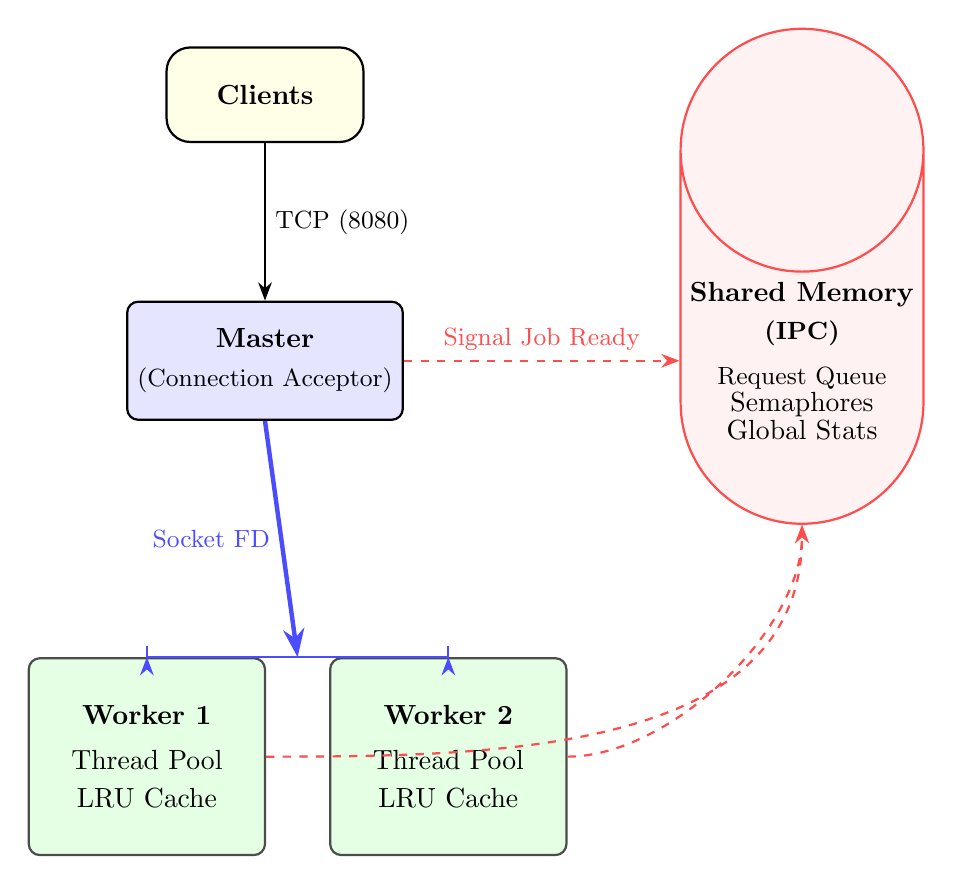
\begin{tikzpicture}[
        process/.style={rectangle, draw=black, thick, fill=blue!10, minimum width=3.5cm, minimum height=1.5cm, align=center, rounded corners, font=\normalsize},
        worker/.style={rectangle, draw=black!70, thick, fill=green!10, minimum width=3cm, minimum height=2.5cm, align=center, rounded corners, font=\normalsize},
        shm/.style={cylinder, shape border rotate=90, draw=red!70, thick, fill=red!5, minimum width=3cm, minimum height=3.5cm, align=center, font=\normalsize},
        comp/.style={rectangle, draw=gray, dashed, fill=white, font=\small, minimum width=2cm, minimum height=0.5cm, align=center},
        cloudnode/.style={rectangle, draw=black, thick, fill=yellow!10, minimum width=2.5cm, minimum height=1.2cm, align=center, rounded corners=0.3cm, font=\normalsize},
        arrow/.style={->, >=Stealth, thick}
    ]

    % Master Process
    \node (master) [process] {\textbf{Master}\\[2pt]\small(Connection Acceptor)};

    % Shared Memory 
    \node (shm) [shm, right=3.5cm of master] {
        \textbf{Shared Memory}\\[2pt]\small\textbf{(IPC)}\\[4pt]
        \small Request Queue\\[-2pt]
        Semaphores\\[-2pt]
        Global Stats
    };
    
    % Workers
    \node (worker1) [worker, below=3cm of master, xshift=-1.5cm] {
        \textbf{Worker 1}\\[4pt]
        Thread Pool\\[2pt]
        LRU Cache
    };

    \node (worker2) [worker, right=0.8cm of worker1] {
        \textbf{Worker 2}\\[4pt]
        Thread Pool\\[2pt]
        LRU Cache
    };

    % Clients
    \node (client) [cloudnode, above=2cm of master] {\textbf{Clients}};

    % Edges
    \draw[arrow] (client) -- node[right, font=\small] {TCP (8080)} (master);

    \draw[arrow, dashed, color=red!70] (master.east) -- (shm.west)
        node[above, midway, font=\small, color=red!70] {Signal Job Ready};

    \draw[arrow, ultra thick, color=blue!70] (master.south) -- 
        node[left, font=\small, color=blue!70] {Socket FD} 
        ($(worker1.north)!0.5!(worker2.north)$);
    
    \draw[arrow, color=blue!70] ($(worker1.north)!0.5!(worker2.north)$) -| (worker1.north);
    \draw[arrow, color=blue!70] ($(worker1.north)!0.5!(worker2.north)$) -| (worker2.north);

    \draw[arrow, dashed, color=red!70] (worker1.east) to[out=0, in=270, looseness=1] (shm.south);
    \draw[arrow, dashed, color=red!70] (worker2.east) to[out=0, in=270, looseness=0.8] (shm.south);

    \end{tikzpicture}
    \caption{System Architecture: Process Model and IPC Coordination}
    \label{fig:arch}
\end{figure}
    
    \subsection{Thread Model}
    
    Within each worker process, a fixed sized pool of threads is created during
    initialization. The pool is managed through a bounded queue protected by a
    \texttt{pthread\_mutex\_t} and a pair of condition variables for signaling.
    Threads block when the queue is empty and wake upon task submission.  
    Each thread handles one complete HTTP request–response cycle before returning
    to the idle state. This design eliminates the overhead of thread creation at
    runtime and maintains steady throughput under heavy load.
    
    \subsection{Coordination and Synchronization}
    
    Interprocess coordination relies on POSIX shared memory and named semaphores.
    Shared memory stores both the connection queue and aggregated statistics,
    while semaphores enforce mutual exclusion and synchronize access between the
    master and workers.  
    Within workers, thread-level synchronization is handled by mutexes and
    condition variables, ensuring safe access to shared structures such as the
    cache and log system. This combination of IPC primitives and in-process
    synchronization guarantees correctness even under high concurrency.
    
    \subsection{Design Rationale}
    
    The architecture separates responsibilities cleanly: the master focuses on
    connection management and system orchestration, while workers specialize in
    request handling. The use of shared memory for lightweight signaling and
    descriptor passing through UNIX domain sockets minimizes communication
    overhead and preserves process isolation.  
    This design yields a scalable, fault-tolerant server capable of leveraging
    multi-core systems effectively while maintaining predictable and stable
    performance.
    
    
    % ----------------------------------------------------------------------
    % 2. SHARED DATA STRUCTURES
    % ----------------------------------------------------------------------
    \section{Shared Data Structures}
    Inter-Process Communication (IPC) between the master and workers relies on
    POSIX shared memory with named semaphores. The shared region holds a
    bounded queue for connection dispatch and a set of global runtime counters.
    
    \subsection{Memory Layout}
    
    Defined in \texttt{shared\_mem.h}, the \texttt{shared\_data\_t} structure
    is allocated by the master process and mapped by all workers.
    
    \begin{lstlisting}[language=C]
    typedef struct {
        request_queue_t queue;   // Connection queue
        server_stats_t  stats;   // Global statistics
    } shared_data_t;
    \end{lstlisting}
    
    Creation uses \texttt{shm\_open()}, \texttt{ftruncate()}, and
    \texttt{mmap()}, with cleanup performed by the master on shutdown
    via \texttt{shm\_unlink()}.
    
    \subsection{Circular Buffer}
    
    The interprocess queue is implemented as a bounded FIFO in shared memory:
    
    \begin{lstlisting}[language=C]
    typedef struct {
        int worker_id;       // Target worker
        int placeholder_fd;  // Marker only (real FD passed via SCM_RIGHTS)
    } connection_item_t;
    
    typedef struct {
        connection_item_t items[MAX_QUEUE_SIZE];
        int front;          // Dequeue index
        int rear;           // Enqueue index
        int count;          // Current occupancy
    } connection_queue_t;
    \end{lstlisting}
    
    \paragraph{Semantics.}\mbox{}\\[-0.2\baselineskip]
    The Master (producer) enqueues a \texttt{connection\_item\_t} selecting the
    \texttt{worker\_id}; the \texttt{placeholder\_fd} is not a transferable descriptor.
    The actual client socket is sent to the chosen Worker over a UNIX domain socket
    using \texttt{SCM\string_RIGHTS}.
    
    \paragraph{Synchronization.}\mbox{}\\[-0.2\baselineskip]
    Enqueue/dequeue follow classical producer--consumer control with named semaphores:
    \texttt{empty\_slots} (free capacity), \texttt{filled\_slots} (pending items),
    and \texttt{queue\_mutex} (exclusive updates of \texttt{front}/\texttt{rear}/\texttt{count}).
    On enqueue: wait \texttt{empty\_slots} $\rightarrow$ lock \texttt{queue\_mutex}
    $\rightarrow$ write \texttt{items[rear]} and advance \texttt{rear} (mod
    \texttt{MAX\_QUEUE\_SIZE}); increment \texttt{count} $\rightarrow$ unlock
    $\rightarrow$ post \texttt{filled\_slots}.  
    On dequeue: wait \texttt{filled\_slots} $\rightarrow$ lock \texttt{queue\_mutex}
    $\rightarrow$ read \texttt{items[front]} and advance \texttt{front}; decrement
    \texttt{count} $\rightarrow$ unlock $\rightarrow$ post \texttt{empty\_slots}.
    This guarantees correctness under concurrent producers/consumers and prevents
    overrun/underrun of the circular buffer.
    
    
    \subsection{Global Statistics}
    
    The \texttt{server\_stats\_t} structure, located in the same region,
    records cumulative server activity.
    
    \begin{lstlisting}[language=C]
    typedef struct {
        long total_requests;          
        long bytes_transferred;        
        long status_200;              
        long status_404;               
        long status_500;            
        int  active_connections;       
        long total_response_time_ms;  
    } server_stats_t;
    \end{lstlisting}
    
    Workers increment these counters under a dedicated semaphore
    (\texttt{stats\_mutex}) to guarantee atomic access.  
    Values are read periodically by monitoring components such as the web
    dashboard and log system.
    
    \subsection{Synchronization Lifecycle}
    
    The master initializes shared memory and all semaphores during startup,
    while workers connect to existing objects.  
    At termination, the master releases all IPC resources, preventing
    persistent semaphores or memory segments.
    
    This design achieves reliable communication and coordinated state
    management with minimal interprocess overhead.
    
    % ----------------------------------------------------------------------
    % 3. SYNCHRONIZATION MECHANISMS
    % ----------------------------------------------------------------------
    \section{Synchronization Mechanisms}
    
    \subsection{Process Synchronization (Named Semaphores)}
    Master and Workers coordinate over a bounded circular queue in shared memory using
    named POSIX semaphores (see \texttt{semaphores.h/.c}, \texttt{shared\_mem.h/.c}):
    
    \begin{itemize}
      \item \textbf{\texttt{empty\_slots}} (\texttt{/ws\_empty}) --- counts free positions in the interprocess queue; the Master (producer) waits when the queue is full.
      \item \textbf{\texttt{filled\_slots}} (\texttt{/ws\_filled}) --- counts pending items. Workers (consumers) wait when the queue is empty.
      \item \textbf{\texttt{queue\_mutex}} (\texttt{/ws\_queue\_mutex}) --- mutual exclusion for updating queue indices (\texttt{front/rear/count}).
      \item \textbf{\texttt{stats\_mutex}} (\texttt{/ws\_stats\_mutex}) --- serializes updates to \texttt{server\_stats\_t} (see \texttt{stats.c}).
      \item \textbf{\texttt{log\_mutex}} (\texttt{/ws\_log\_mutex}) --- serializes log writes across processes.
    \end{itemize}
    
    Producer path (in \texttt{master.c}): wait \texttt{empty\_slots} $\rightarrow$ lock \texttt{queue\_mutex} $\rightarrow$ enqueue $\rightarrow$ unlock $\rightarrow$ post \texttt{filled\_slots}.  
    Consumer path (in \texttt{worker.c}): wait \texttt{filled\_slots} $\rightarrow$ lock \texttt{queue\_mutex} $\rightarrow$ dequeue $\rightarrow$ unlock $\rightarrow$ post \texttt{empty\_slots}.
    
        \begin{figure}[H]
nd{document}
